\documentclass{article}
\usepackage[left=25mm,top=1in,bottom=0.5in]{geometry}
\usepackage{fancyhdr}
\usepackage{extramarks}
\usepackage{amsmath}
\usepackage{amsthm}
\usepackage{amsfonts}
\usepackage{tikz}
\usepackage[plain]{algorithm}
\usepackage{algpseudocode}
\usepackage{listings}
\usepackage{minted}
\usepackage{graphicx}
\usepackage[dvipsnames]{xcolor}
\graphicspath{ {./} }
\definecolor{codegreen}{rgb}{0,0.6,0}
\definecolor{codegray}{rgb}{0.5,0.5,0.5}
\definecolor{codepurple}{rgb}{0.58,0,0.82}
\definecolor{backcolour}{rgb}{0.95,0.95,0.92}

\lstdefinestyle{mystyle}{
    backgroundcolor=\color{backcolour},
    commentstyle=\color{codegreen},
    keywordstyle=\color{magenta},
    numberstyle=\tiny\color{codegray},
    stringstyle=\color{codepurple},
    basicstyle=\ttfamily\footnotesize,
    breakatwhitespace=false,         
    breaklines=true,                 
    captionpos=b,                    
    keepspaces=true,                 
    numbers=left,                    
    numbersep=5pt,                  
    showspaces=false,                
    showstringspaces=false,
    showtabs=false,                  
    tabsize=2
}
\pagestyle{fancy}
\lhead{DEEKSHA ARORA}
\chead{CS 685}
%\rhead{\firstxmark}
\lfoot{\lastxmark}
\cfoot{\thepage}

\title{CS 685 (Data Mining)
Assignment 2}
\author{\textbf{DEEKSHA ARORA} \\ Roll No. 20111017}
\date{Due date: November 20, 2020 \\ Instructor: Prof. Arnab Bhattacharya}

\newcommand{\enterProblemHeader}[1]{
    \nobreak\extramarks{}{Problem \arabic{#1} continued on next page\ldots}\nobreak{}
    \nobreak\extramarks{Problem \arabic{#1} (continued)}{Problem \arabic{#1} continued on next page\ldots}\nobreak{}
}

\newcommand{\exitProblemHeader}[1]{
    \nobreak\extramarks{Problem \arabic{#1} (continued)}{Problem \arabic{#1} continued on next page\ldots}\nobreak{}
    \stepcounter{#1}
    \nobreak\extramarks{Problem \arabic{#1}}{}\nobreak{}
}

\setcounter{secnumdepth}{0}
\newcounter{partCounter}
\newcounter{homeworkProblemCounter}
\setcounter{homeworkProblemCounter}{1}
\nobreak\extramarks{Problem \arabic{homeworkProblemCounter}}{}\nobreak{}

\newenvironment{homeworkProblem}[1][-1]{
    \ifnum#1>0
        \setcounter{homeworkProblemCounter}{#1}
    \fi
    \section{Problem \arabic{homeworkProblemCounter}}
    \setcounter{partCounter}{1}
    \enterProblemHeader{homeworkProblemCounter}
}{
    \exitProblemHeader{homeworkProblemCounter}
}

\begin{document}

\maketitle
\pagebreak
\lstset{style=mystyle}
\begin{center}
\section{{REPORT}}
\end{center}
\subsection{INTRODUCTION}
Wikispeedia is a human-computation game where a user can navigate from one article to another through links present within the article. The user is given two Wikipedia articles and he is required to reach the destination article from source article using minimum clicks. The player is unknown of the shortest path between the two articles and rather finds an intuitive path. This intuition helps in learning the common sense knowledge by using the history of paths followed by the human. This knowledge is important as it helps in analyzing the human navigation patterns and gives a clear picture of how humans reason about complex networks. This helps in building more human-friendly and intuitively navigable information systems. \\
This assignment uses the data collected through Wikispeedia (retrieved from Stanford's SNAP lab) which uses a condensed version of Wikipedia articles (4,604 articles).
\subsection{RESULT ANALYSIS}
\begin{itemize}
    \item \textbf{Question 1-} The article names present in articles.tsv file are URL-encoded. These articles names are decoded and assigned ID from A0001 to A4604.
    \item \textbf{Question 2-}  There are a total of 146 categories to which an article can belong. All the article categories in Wikispeedia form a tree with $subject$ as the root node. These categories are assigned IDs from C0001 to C0146 in Breadth First order.
    \item \textbf{Question 3-} Each article is mapped to all the possible categories to which it can belong. This reveals that some articles belong to one category, some belong to more than one category and there are some articles which do not belong to any category. It is observed that the articles are mapped to the leaf nodes of the category tree. The articles which do not belong to any category are mapped to the root node ($subject$).
    \item \textbf{Question 4-} A directed graph is constructed with articles(Article ID) as nodes and the links between articles as edges. An edge in this directed graph from node n1 to n2 shows that there is a hyperlink in article n1 to reach article n2. To construct this graph, shortest-path-distance-matrix.txt file is used. The articles which have distance between them as 1 are connected directly with an edge in the directed graph.\\ 
    The edges in the output file (edges.csv) are represented in edge list format. There are a total of 119,772 edges in the directed graph.
    \item \textbf{Question 5-} Considering the graph as \textbf{undirected}, we get 2 connected components and 12 isolated nodes. The larger component has $4589$ nodes and $106,534$ edges while the smaller component has $3$ nodes and $3$ edges. The diameter of these connected components is 5 and 1 respectively. Since the diameter of a graph represents the length of longest shortest path, so this shows that for any $2$ articles in the connected components(of undirected graph) there exists a path between them with a maximum of 5 edges.
    \item \textbf{Question 6-} The Wikispeedia game allows participants to backtrack without any penalty, thus the participant can re-visit the previous article if he thinks that he has made a wrong move. These regret nodes are represented by `$<$' . Since humans are bound to make mistake during navigation in such complex networks, so we have divided our analysis in two parts: one which counts the regret nodes in path length and the other which doesn't count the regret nodes in path length. If we ignore the back clicks in human path, it is equivalent to have path with no mistakes and therefore the ratio of length of human path to shortest path improves.\\
    \\
    Methodology for computing the length of human traversed path in the above mentioned two analysis is as follows:\\
    \\
    \textbf{1. With back clicks: }In this method, length of human path is: \\
    \centerline{count of all visited articles or nodes(including regret nodes) - 1}\\
    \\
    \textbf{2. Without back clicks: }In this method, if the user backtracks from a node then that particular node and the corresponding edges are not considered in the path length. The formula for path length is:\\
    \centerline{count of all visited nodes(including regret nodes) - 2 x number of regret nodes}\\
    \\
    The shortest path between any two articles is the minimum number of clicks(edges) required to reach the destination article from the source article.\\
    \\
    The following example will help in better understanding of path length with back clicks, without back clicks and shortest path.
\\
\begin{figure}[h]
\centerline{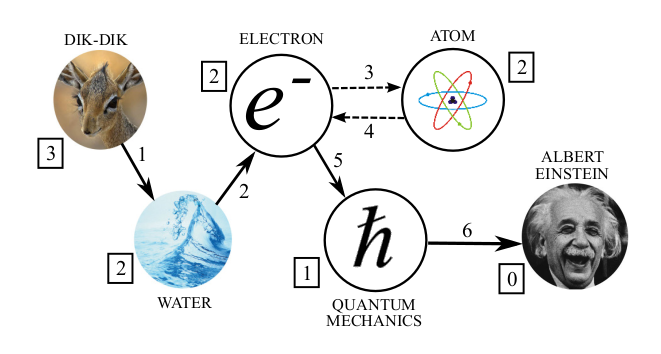
\includegraphics[scale=0.7]{photo1.png}}
\caption{Wikispeedia example path between the articles DIK-DIK and ALBERT EINSTEIN}
\label{fig}
\end{figure}\\
In the above figure, the nodes represent Wikipedia articles and edges represent the hyperlinks clicked by the human. Edge labels indicate the order of clicks and the framed numbers represent the shortest-path length to the target. The dotted edges represent that the user backtracked from article ``Atom" to ``Electron". So, in this case, the length of human path considering the back clicks will be 6 and without considering back clicks will be 4. One of several possible shortest paths would be $<$ DIK-DIK , WATER , GERMANY , ALBERT EINSTEIN $>$ with shortest path length as 3.
\item \textbf{Question 7- }In this part, we have found the percentage of human paths that have path length: exactly the same as the shortest path, that have path 1 to 10 more than the shortest path (each separately), that have path length 11 or more than the shortest path. The results have shown that very few participants followed the shortest path to reach the destination article and mostly everyone followed intuition to reach the destination article.
\item \textbf{Question 8- }Here for each finished human path (without back links) and its corresponding shortest
path we have found the number of paths where each category is traversed and number of times each category is traversed (i.e. counted each category multiple times if it is visited multiple times in a path). To know the shortest path between any two categories I used NetworkX library. The articles which didn't belong to any category were assigned $subject$ category.\\
This helped in analyzing the frequently visited categories and get hold of the relative frequencies of their visit. The analysis shows that $subject.Countries$ is the most frequently visited category. \\
\begin{figure}[h]
\centerline{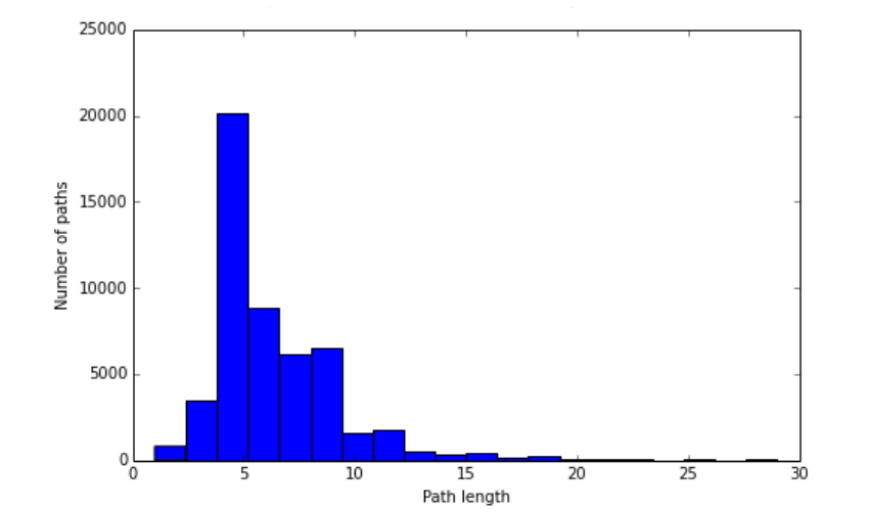
\includegraphics[scale=0.45]{photo2.png}}
\caption{Histogram of Human path lengths with average 6.28}
\label{fig}
\end{figure}\\
\begin{figure}[h]
\centerline{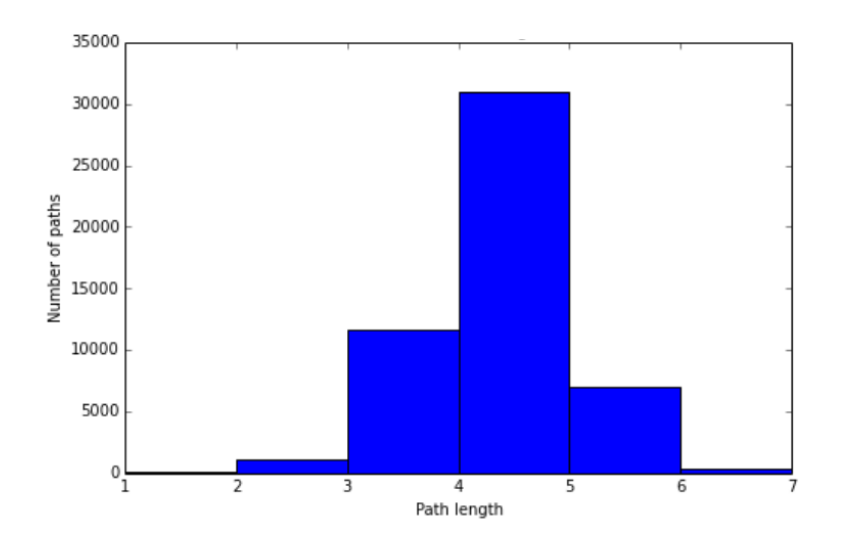
\includegraphics[scale=0.4]{photo3.png}}
\caption{Histogram of shortest path lengths with average 3.88}
\label{fig}
\end{figure}
\newpage
\item \textbf{Question 9- }In this part, we considered even the subcategories to which an article belongs. The analysis shows that subject is the most frequently visited category because  it is the root of subcategory tree and thus every article belongs to this category. The second most visited category is $subject.Geography$.
\item \textbf{Question 10- }In this part, for every unfinished and finished path we have found the source and destination category pair and then the percentage of finished and unfinished paths for each source-destination category pair. The analysis gave a broad idea of whether the participant was able to reach an article in the destination category from the specified article in source category.
\item \textbf{Question 11- }In this part, for every source-destination category pair we found the average ratio of length of human(without back clicks) paths to shortest paths. The results showed the difference between the path length followed by a human and the shortest path for each category pair. The category pair $subject.Everyday\_life.Films, subject.Language\_and\_literature.Literature\_types$ has the largest human to shortest path ratio of 17.66.
\end{itemize}

\section{CONCLUSION}
Using the analysis done so far, we can derive the following conclusions:
\begin{itemize}
    \item One connected component has a large chunk of articles i.e. 4589 articles in it. This shows that there is no such thing as an isolated piece of knowledge. All the bits of information are connected to each other in a complex network of information
    \item Humans very rarely follow shortest paths and rather use intuition and common sense knowledge to reach their destination.
    \item 22.37\% of humans managed to find the shortest path even without having any knowledge of Wikispeedia's structure. This shows that humans do manage to find the shortest paths by using their background knowledge and thus determine which hyperlink in the present article is most promising and will reduce the distance to target article.
    \item The back clicks present in the human paths show the uncertainity in human behavior. Humans take a particular path and later realise that this path may not reach the target and thus they backtrack.
    \item The human paths reveal which articles according to the common sense or background knowledge of the participant can be inferred as related to the target article. This helps in improving the human interactive information systems by providing hyperlinks from these articles to the target articles for convenience of the user. 
    \end{itemize}
\end{document}
